\documentclass[a4paper, 12pt]{article}
% packages
\usepackage{amssymb}
\usepackage[fleqn]{mathtools}
\usepackage{tikz}
\usepackage{enumerate}
\usepackage{bussproofs}
\usepackage{xcolor}
\usepackage[margin=1.3cm]{geometry}
\usepackage{logicproof}
\usepackage{diagbox}
\usepackage{listings}
\usepackage{graphicx}
\usepackage{lstautogobble}
\usepackage{hyperref}
\usepackage{multirow}
\usetikzlibrary{arrows, shapes.gates.logic.US, circuits.logic.US, calc, automata, positioning}

% shorthand for verbatim
\catcode`~=\active
\def~#1~{\texttt{#1}}

% code listing
\lstdefinestyle{main}{
    numberstyle=\tiny,
    breaklines=true,
    showspaces=false,
    showstringspaces=false,
    tabsize=2,
    numbers=left,
    basicstyle=\ttfamily,
    columns=fixed,
    fontadjust=true,
    basewidth=0.5em,
    autogobble,
    xleftmargin=3.0ex,
    mathescape=true
}
\newcommand{\dollar}{\mbox{\textdollar}} %
\lstset{style=main}

% augmented matrix
\makeatletter
\renewcommand*\env@matrix[1][*\c@MaxMatrixCols c]{%
\hskip -\arraycolsep
\let\@ifnextchar\new@ifnextchar
\array{#1}}
\makeatother

% ceiling / floor
\DeclarePairedDelimiter{\ceil}{\lceil}{\rceil}
\DeclarePairedDelimiter{\floor}{\lfloor}{\rfloor}

% custom commands
\newcommand{\indefint}[2]{\int #1 \, \mathrm{d}#2}
\newcommand{\defint}[4]{\int_{#1}^{#2} #3 \, \mathrm{d}#4}
\newcommand{\dif}[2]{\frac{\mathrm{d}#1}{\mathrm{d}#2}}
\newcommand{\limit}[2]{\displaystyle{\lim_{#1 \to #2}}}
\newcommand{\summation}[3]{\sum\limits_{#1}^{#2} #3}
\newcommand{\intbracket}[3]{\left[#3\right]_{#1}^{#2}}

\newcommand{\powerset}[0]{\wp}
\renewcommand{\emptyset}[0]{\varnothing}

\newcommand{\unaryproof}[2]{\AxiomC{#1} \UnaryInfC{#2} \DisplayProof}
\newcommand{\binaryproof}[3]{\AxiomC{#1} \AxiomC{#2} \BinaryInfC{#3} \DisplayProof}
\newcommand{\trinaryproof}[4]{\AxiomC{#1} \AxiomC{#2} \AxiomC{#3} \TrinaryInfC{#4} \DisplayProof}

% no indent
\setlength\parindent{0pt}

% reasoning proofs
\usepackage{ltablex}
\usepackage{environ}
\keepXColumns
\NewEnviron{reasoning}{
    \begin{tabularx}{\textwidth}{rlX}
        \BODY
    \end{tabularx}
}
\newcommand{\proofline}[3]{$(#1)$ & $#2$ & \hfill #3 \smallskip \\}
\newcommand{\proofarbitrary}[1]{& take arbitrary $#1$ \smallskip \\}
\newcommand{\prooftext}[1]{\multicolumn{3}{l}{#1} \smallskip \\}
\newcommand{\proofmath}[3]{$#1$ & = $#2$ & \hfill #3 \smallskip \\}
\newcommand{\prooftherefore}[1]{& $\therefore #1$ \smallskip \\}
\newcommand{\proofbc}[0]{\prooftext{\textbf{Base Case}}}
\newcommand{\proofis}[0]{\prooftext{\textbf{Inductive Step}}}

% reasoning er diagrams
\newcommand{\nattribute}[4]{
    \node[draw, state, inner sep=0cm, minimum size=0.2cm, label=#3:{#4}] (#1) at (#2) {};
}
\newcommand{\mattribute}[4]{
    \node[draw, state, accepting, inner sep=0cm, minimum size=0.2cm, label=#3:{#4}] (#1) at (#2) {};
}
\newcommand{\dattribute}[4]{
    \node[draw, state, dashed, inner sep=0cm, minimum size=0.2cm, label=#3:{#4}] (#1) at (#2) {};
}
\newcommand{\entity}[4]{
    \node[] (#1-c) at (#2, #3) {#4};
    \node[inner sep=0cm] (#1-l) at ($(#1-c) + (-1, 0)$) {};
    \node[inner sep=0cm] (#1-r) at ($(#1-c) + (1, 0)$) {};
    \node[inner sep=0cm] (#1-u) at ($(#1-c) + (0, 0.5)$) {};
    \node[inner sep=0cm] (#1-d) at ($(#1-c) + (0, -0.5)$) {};
    \draw
    ($(#1-c) + (-1, 0.5)$) -- ($(#1-c) + (1, 0.5)$) -- ($(#1-c) + (1, -0.5)$) -- ($(#1-c) + (-1, -0.5)$) -- cycle;
}
\newcommand{\relationship}[4]{
    \node[] (#1-c) at (#2, #3) {#4};
    \node[inner sep=0cm] (#1-l) at ($(#1-c) + (-1, 0)$) {};
    \node[inner sep=0cm] (#1-r) at ($(#1-c) + (1, 0)$) {};
    \node[inner sep=0cm] (#1-u) at ($(#1-c) + (0, 1)$) {};
    \node[inner sep=0cm] (#1-d) at ($(#1-c) + (0, -1)$) {};
    \draw
    ($(#1-c) + (-1, 0)$) -- ($(#1-c) + (0, 1)$) -- ($(#1-c) + (1, 0)$) -- ($(#1-c) + (0, -1)$) -- cycle;
}

% actual document
\begin{document}
    \section*{CO130 - Databases}
        \subsection*{Prelude}
            The content discussed here is part of CO130 - Databases (Computing MEng); taught by Thomas Heinis, in Imperial College London during the academic year 2018/19. The notes are written for my personal use, and have no guarantee of being correct (although I hope it is, for my own sake).
        \subsection*{Material Order}
            These notes are primarily based off the slides on CATe. This is the order in which they are uploaded (and I'd assume the order in which they are taught).
            \begin{enumerate}[1.]
                \itemsep0em
                \item \textit{Introduction.pdf}
                \item \textit{ER Modelling.pdf}
                \item \textit{ER to RM.pdf}
                \item \textit{Relational Algebra.pdf}
                \item \textit{Tutorial ER.pdf}
                \item \textit{Tutorial Translation.pdf}
                \item \textit{Relational Algebra.pdf}
                \item \textit{Functional Dependencies.pdf}
                \item \textit{Tutorial Relational Algebra.pdf}
                \item \textit{Normalisation.pdf}
                \item \textit{SQL.pdf}
                \item \textit{Data Definition.pdf}
                \item \textit{Data Manipulation.pdf}
                \item \textit{Advanced SQL.pdf}
                \item \textit{Functional Dependency Tutorial.pdf}
                \item \textit{Transactions.pdf}
                \item \textit{SQL Tutorial.pdf}
                \item \textit{Storage.pdf}
                \item \textit{Indexing.pdf}
                \item \textit{NoSQL.pdf}
                \item \textit{MapReduce.pdf}
            \end{enumerate}
        \subsection*{Introduction}
            We use databases as it's more organised; hence it's easier to model and manage. It's more efficient, as it's fast to search, and update, and integration allows us to minimise data duplication. Concurrent (and therefore multi-user) access allows multiple people to access the database at the same time (will require some techniques).
            \medskip

            \textbf{Transactions} are sequences of database actions that execute in a coherent, and reliable way - the classical properties are \textbf{ACID}. Consider the two transactions ~T1~: $A = A - 100; B = B + 100$, and ~T2~: $B = B - 100; A = A + 100$, we can observe ACID properties as follows;
            \begin{itemize}
                \itemsep0em
                \item \textbf{atomicity} \hfill if one part of a transaction fails, the entire transaction fails
                    \subitem on completion of ~T1~, either $A^\prime = A - 100$, and $B^\prime = B + 100$, or $A^\prime = A$, and $B^\prime = B$, where the former is a successful transaction, and the latter is in the case of a failure.
                \item \textbf{consistency} \hfill transactions don't leave the database in an inconsistent state
                    \subitem the sum of the balances must remain the same, such that $A^\prime + B^\prime = A + B$; we can also have more constraints such as keeping balances positive, or limiting the amount a transfer can do at once
                \item \textbf{isolation} \hfill transactions run as if no other transactions are running (may need to wait)
                    \subitem given the two concurrent transactions ~T1~, and ~T2~, one has to be completed before the other can start
                \item \textbf{durability} \hfill results of successful transactions aren't lost on system failure
                    \subitem the new values, $A^\prime$, and $B^\prime$ must persist if the transaction completes, even if the system fails (disk failure etc.)
            \end{itemize}
            A \textbf{Database Management System (DMBS)} creates new databases via a \textbf{Data Definition Language (DDL)}, which specifies the structure (\textbf{schema}). It also queries, and manipulates through a \textbf{Data Manipulation Language (DML)}. Examples of this include \textit{PostgreSQL}, \textit{MySQL}, \textit{SQLite}, and can also fall under \textit{NoSQL}, however SQL remains as the most widespread technology (as of writing this).
            \medskip

            It lets us define, query, and manipulate databases with a high-levle declarative language (\textbf{Structured Query Language}). It's standardised by the ISO, but each DBMS implements its own variation of the standards, which may be costly if it's complex.
            \subsubsection*{Relational Model}
                Consider the following model, represented as a table;
                \begin{center}
                    \begin{tabular}{|c|c|c|c|c|}
                        \hline
                        heading & ~title:string~ & ~year:int~ & ~length:int~ & ~genre:string~ \\
                        \hline
                        \hline
                        \multirow{3}{*}{body} & Gone with the Wind & 1939 & 231 & Drama \\
                        \cline{2-5}
                        & Star Wars & 1977 & 124 & Science Fiction \\
                        \cline{2-5}
                        & Wayne's World & 1992 & 95 & Comedy \\
                        \hline
                    \end{tabular}
                \end{center}
                We have the columns be the attribute, with the top row being the heading, and the rest being the body. The attributes are in the format ~name:type~. The rows (of the body) are referred to as tuples. A relation is the heading as well as the body (the entire table). The heading is an \textbf{unordered set} of attributes, and an attribute is the name as well as the type (typically indivisible types). The body is an unordered set of tuples, and a tuple is the set of attribute values. The schema is for the entire relation is the name of the relation, and the heading, in this case, we'd have; ~movies(title:string, year:int, length:int, genre:string)~, and a database is a collection of relations. A schema for a database is the schemas for all relations.
                \medskip

                In mathematics, with a set of sets; $S_1, S_2, ..., S_n$, a relation $R$ is a set of tuples $T_1, T_2, ..., T_n$, where $T_k \in S_k$, therefore $R \subset S_1 \times S_2 \times ... \times S_n$. As the idea of relations stems from set theory, it's important to note that the order in which we represent the attributes, and tuples in unimportant. In the Relational model we have \textbf{attributed} tuples, rather than \textbf{ordered}; $R$ is the set of tuples ($A_1:S_1=T_1, ..., A_n:S_n=T_n$), with $T_k \in S_k$. It's important to note that relations aren't 2-dimensional tables, even though it's more convineient to draw it on paper. We should instead consider them as a set of $n$-dimensional values, such that we have (~title:string~=StarWars, ~year:int~=1997, ~length:int~=127, ~genre:string~=ScienceFiction), as a 4-dimensional movie value.
        \subsection*{Entity Relationship Modelling}
            When a new database is being developed, it's important to try and model the real-world situation, instead of trying to refine it into an implementation, such as a relational model. In Entity-Relationship modelling, we try to create a diagram which represents the information needed for the database (the Entity Relationship Diagram). As there is no universally accepting notation for ER diagrams, we will use the following notation;
            \begin{center}
                \begin{tabularx}{\textwidth}{|c|X|c|}
                    \hline
                    type & description & shape \\
                    \hline
                    \hline
                    entity sets & a set of distinguisable entries that share the same set of properties, can be physical (a room etc.), an event (flight, sale, etc.) - they normally correspond to nouns & rectangle \\
                    \hline
                    relationship sets & captures how \textbf{two or more} entity sets are related (e.g. owns, tutors), we can also have more than one relationship set between entity sets, and they can also have a relationship set on the same entity - they sometimes correspond to verbs & diamonds \\
                    \hline
                    attributes & properties of an entity; relationship sets can also have attributes, and primary keys are underlined & small circles \\
                    \hline
                \end{tabularx}
                \vspace{-1.5\baselineskip}
            \end{center}
            The movie example is represented below. Note that I've also extended it to contain different types of complex attributes. You can see that the address field is subdivided into number, and postcode, we have a multivalued attribute in phones, and a derived attribute in age (can be calculated from date of birth)
            \begin{center}
                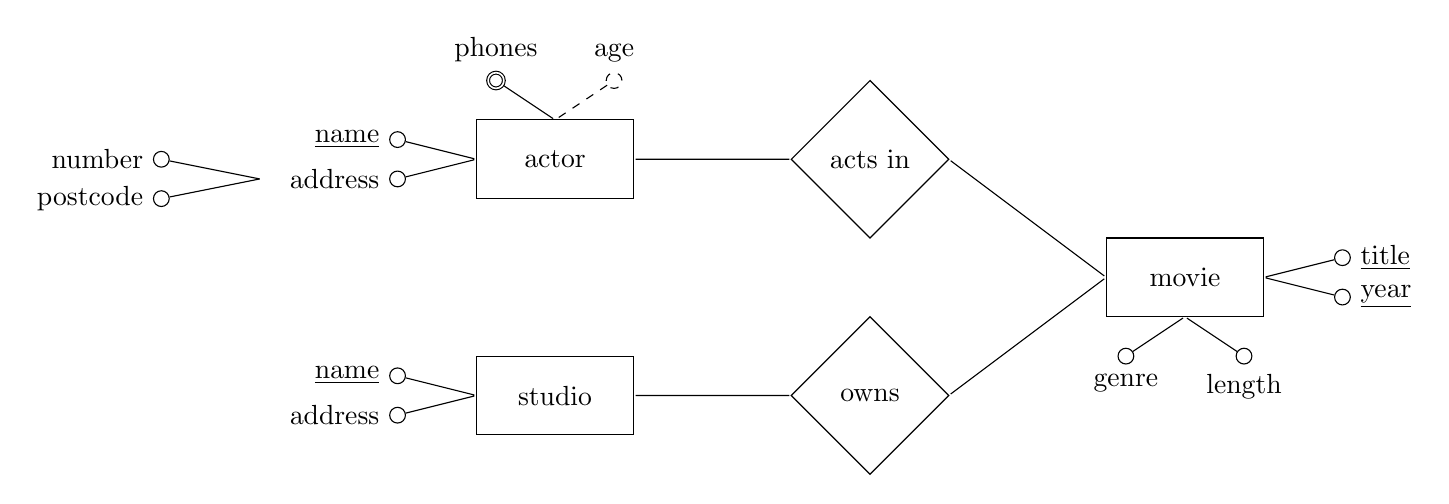
\begin{tikzpicture}
                    \entity{actor}{0}{0}{actor}
                    \entity{studio}{0}{-3}{studio}
                    \relationship{actsin}{4}{0}{acts in}
                    \relationship{owns}{4}{-3}{owns}
                    \entity{movie}{8}{-1.5}{movie}
                    \nattribute{nactor}{-2, 0.25}{left}{\underline{name}}
                    \nattribute{aactor}{-2, -0.25}{left}{address}
                    \mattribute{phones}{-0.75, 1}{above}{phones}
                    \dattribute{age}{0.75, 1}{above}{age}
                    \nattribute{nstudio}{-2, -2.75}{left}{\underline{name}}
                    \nattribute{astudio}{-2, -3.25}{left}{address}
                    \nattribute{mtitle}{10, -1.25}{right}{\underline{title}}
                    \nattribute{myear}{10, -1.75}{right}{\underline{year}}
                    \nattribute{mgenre}{7.25, -2.5}{below}{genre}
                    \nattribute{mlength}{8.75, -2.5}{below}{length}
                    \nattribute{anumber}{-5, 0}{left}{number}
                    \nattribute{apostcode}{-5, -0.5}{left}{postcode}
                    \draw
                    (nactor) -- (actor-l)
                    (aactor) -- (actor-l)
                    (phones) -- (actor-u)
                    (age) edge[dashed] (actor-u)
                    (nstudio) -- (studio-l)
                    (astudio) -- (studio-l)
                    (actor-r) -- (actsin-l)
                    (studio-r) -- (owns-l)
                    (actsin-r) -- (movie-l)
                    (owns-r) -- (movie-l)
                    (movie-r) -- (mtitle)
                    (movie-r) -- (myear)
                    (movie-d) -- (mgenre)
                    (movie-d) -- (mlength)
                    (anumber) -- (-3.75, -0.25)
                    (apostcode) -- (-3.75, -0.25);
                \end{tikzpicture}
            \end{center}
\end{document}
